\documentclass[../report.tex]{subfiles}

\begin{document}

\begin{figure}
\centering
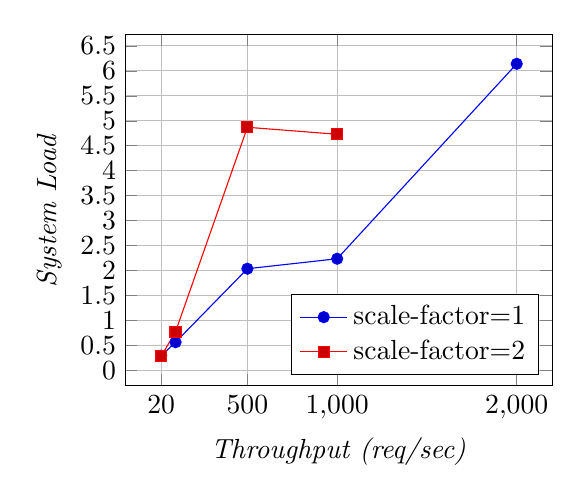
\begin{tikzpicture}[baseline]
    % \begin{axis}[width=7cm, xlabel=\emph{Throughput (req/sec)}, ylabel=\emph{System Load}, ylabel near ticks, grid=major, legend pos=south east, nodes near coords, every node near coord/.append style={font=\footnotesize}, every node near coord/.append style={yshift=-0.5cm}]
    \begin{axis}[width=7cm, xlabel=\emph{Throughput (req/sec)}, ylabel=\emph{System Load}, ylabel near ticks, grid=major, legend pos=south east, ytick distance=0.5, xtick={20, 500, 1000, 2000}]
        \addplot coordinates {
            (2000,6.14) (1000,2.24) (500,2.04) (100,0.57) (20,0.3)
        };
        \addlegendentry{scale-factor=1}

        \addplot coordinates {
            (1000,4.73) (500,4.87) (100,0.78) (20,0.29)
        };
        \addlegendentry{scale-factor=2}
    \end{axis}
\end{tikzpicture}
\label{fig:oltp_pg_load}
\caption{System load during Postgres's TPC-C benchmark}
\end{figure}

% \begin{tikzpicture}[baseline]
%     \begin{axis}[title=CockroachDB, xlabel=\emph{Throughput (req/sec)}, ylabel=\emph{System Load}, ylabel near ticks, grid=major, legend pos=south east, nodes near coords, every node near coord/.append style={font=\footnotesize}, every node near coord/.append style={yshift=-0.5cm}]
%         \addlegendentry{scale-factor=1}
%         \addlegendentry{scale-factor=2}
%     \end{axis}
% \end{tikzpicture}

\end{document}
